\documentclass[12pt,letterpaper]{article}
\usepackage{amsmath,amsthm,amsfonts,amssymb,amscd}
\usepackage{fullpage}
\usepackage{graphicx}
\usepackage{lastpage}
\usepackage{listings}
\lstset{
	numbers=left,
	numbersep=5pt,
	stepnumber=1,
	tabsize=2,
	showstringspaces=false
}
\usepackage{enumerate}
\usepackage{fancyhdr}
\usepackage{hyperref}
\usepackage{mathrsfs}
\usepackage{cancel}
\usepackage{xcolor}
\usepackage[margin=3cm]{geometry}
\setlength{\parindent}{0.0in}
\setlength{\parskip}{0.05in}

% Edit these as appropriate
\newcommand\course{STA561/CS571}
\newcommand\semester{Fall 2013}     % <-- current semester
\newcommand\hwnum{6}                  % <-- homework number
\newcommand\yourname{Matt Dickenson} % <-- your name
\newcommand\login{mcd31}           % <-- your NetID
\newcommand\hwdate{Due: 4 November, 2013}           % <-- HW due date

\newenvironment{answer}[1]{
  \subsubsection*{Problem #1}
}


\pagestyle{fancyplain}
\headheight 35pt
\lhead{\yourname\ \texttt{\login}\\\course\ --- \semester}
\chead{\textbf{\Large Homework \hwnum}}
\rhead{\hwdate}
\headsep 10pt

\begin{document}

\noindent \emph{Homework Notes:} I did not work with anyone else on this homework or refer to resources other than the course notes, textbook, and course Piazza page.

\begin{answer}{1}

\paragraph{A} 

To update the sample of $\mu_k$ at iteration $m+1$, we can sample $\mu_{k,m+1} \sim Unif(l,u)$ where $l=min(0, \mu_k-\epsilon)$ and $u=max(5, \mu_k+\epsilon)$. The prevents us from sampling outside the range defined by the prior. In my samples, I set the `step' $\epsilon=0.1$. 

The MH acceptance probability is the ratio of the likelihood of the new and old samples: $p(keep)={\mathcal{L}(X|\mu_{m+1}) \over \mathcal{L}(X|\mu_{m})}$ (or 1, if the ratio is greater than 1). 


\paragraph{B}  
% Why do we choose to perform MH here instead of a Gibbs sample step?

We chose to perform Metropolis-Hastings rather than a Gibbs sample step because we need to sample $\mu_k$ for all $k$ simultaneously.  Moreover, we cannot sample from the the conditional probability $p(\mu_k | x, z, \Sigma)$, which would be needed for the Gibbs step. 


\paragraph{C} 

I ran 500 rounds of burn-in and 3,000 iterations of sampling. Parameters were initialized as:

\lstinputlisting[language=R, caption=R Code for Initial Parameters, firstline=37, lastline=59, firstnumber=1]{cs571-hw6.r}

The following code runs the burn-in and sampling iterations: 
\lstinputlisting[language=R, caption=R Code for MH, firstline=63, lastline=109, firstnumber=25]{cs571-hw6.r}

\paragraph{D}

% Show the log likelihood trace for three different runs of the sampler starting at three different points on the data you downloaded.

Figure \ref{traceplots} shows the log likelihood trace for three different runs of the sampler using three different (randomly chosen) starting points.

\begin{figure}[h!]
\begin{center}
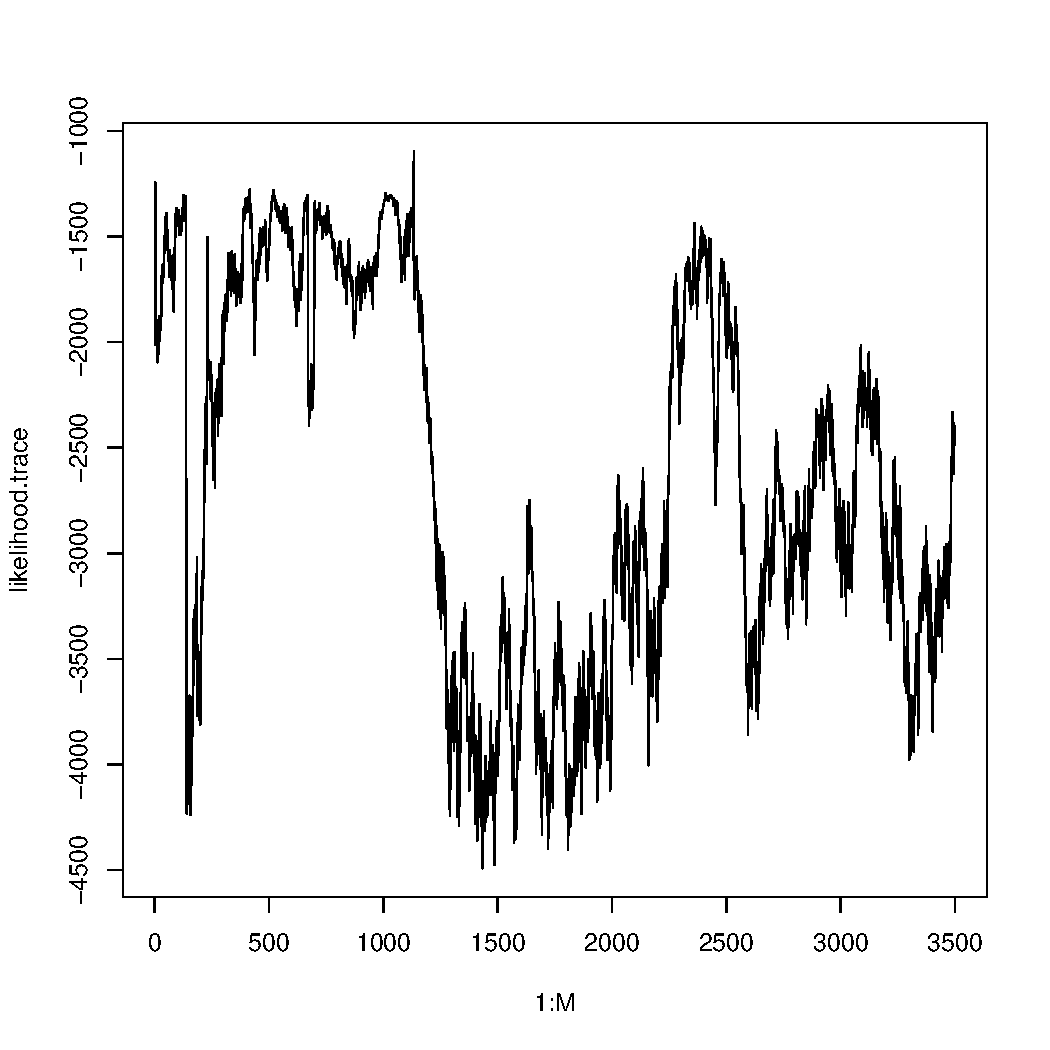
\includegraphics[scale=0.4]{likelihood1.pdf}
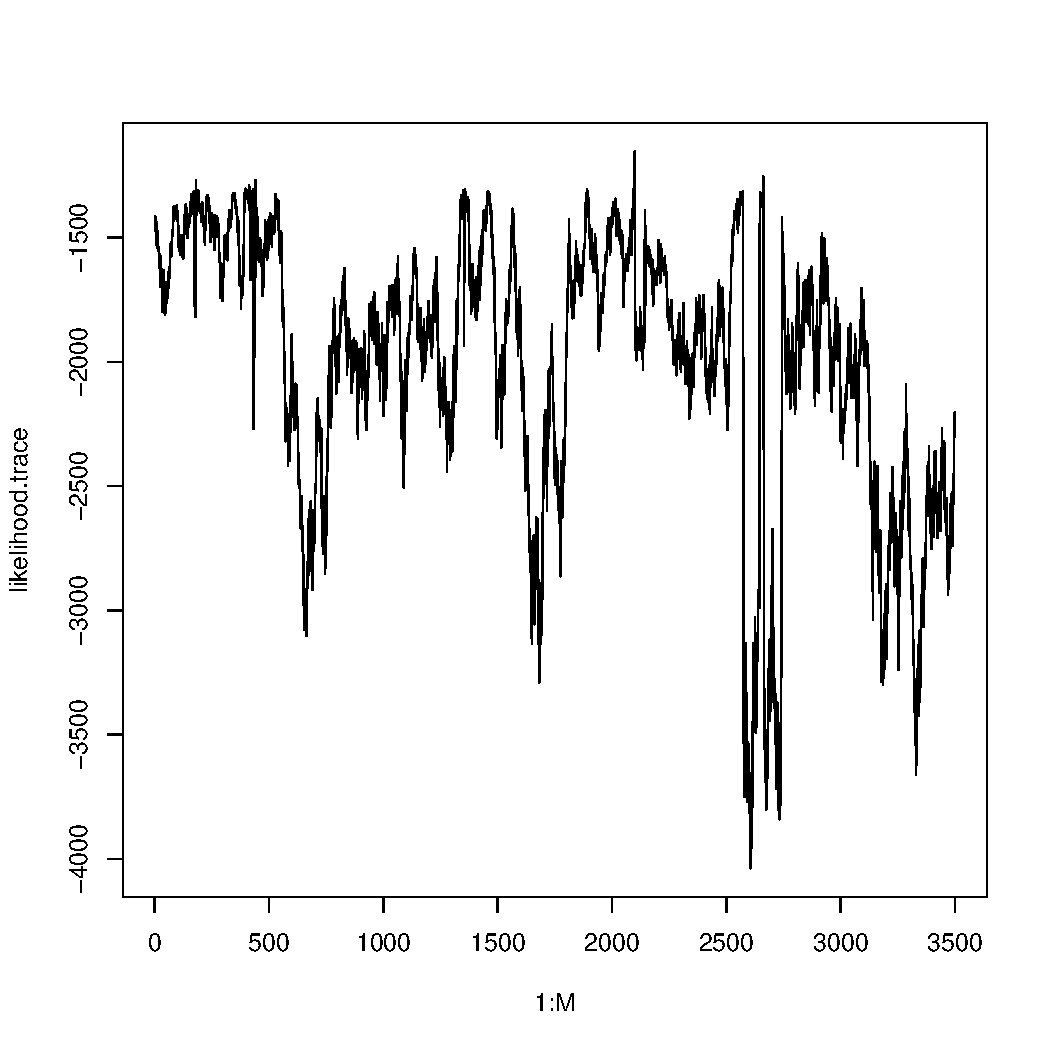
\includegraphics[scale=0.4]{likelihood2.pdf}
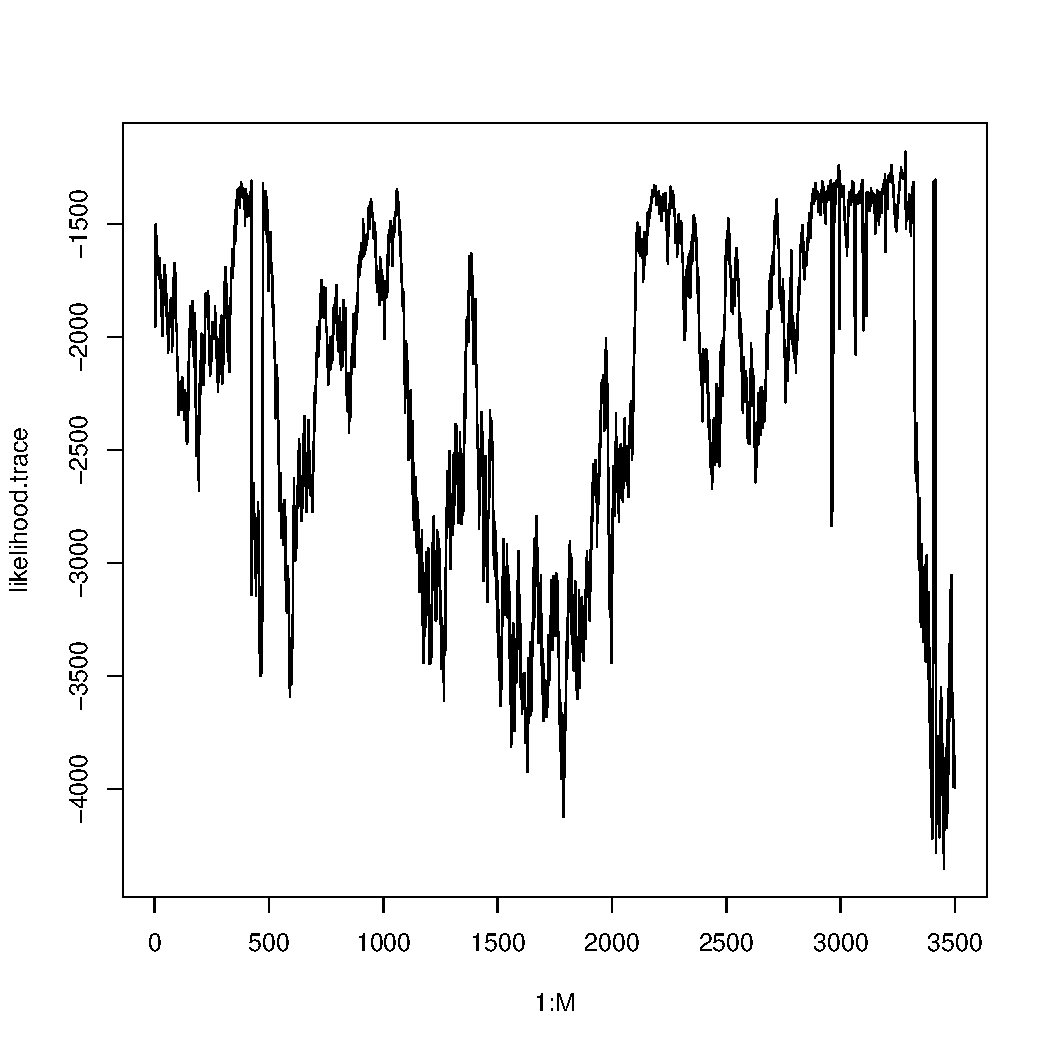
\includegraphics[scale=0.4]{likelihood3.pdf}
\caption{Traceplot of Likelihood for Three Starting Points}
\label{traceplots}
\end{center}
\end{figure}

\paragraph{E}

% Plot a histogram of the posterior samples for each mean parameter for a single run (after burn-in). Write one sentence about what this means. Did label switching occur?

Figure \ref{post-samps} presents histograms of the posterior samples for each mean parameter from a single run (after burn-in).  It appears that $K=2$ is a reasonable fit for the data, with $\mu \approx (1.5, 3)$. Label switching did not occur in these samples. 

\begin{figure}[h!]
\begin{center}
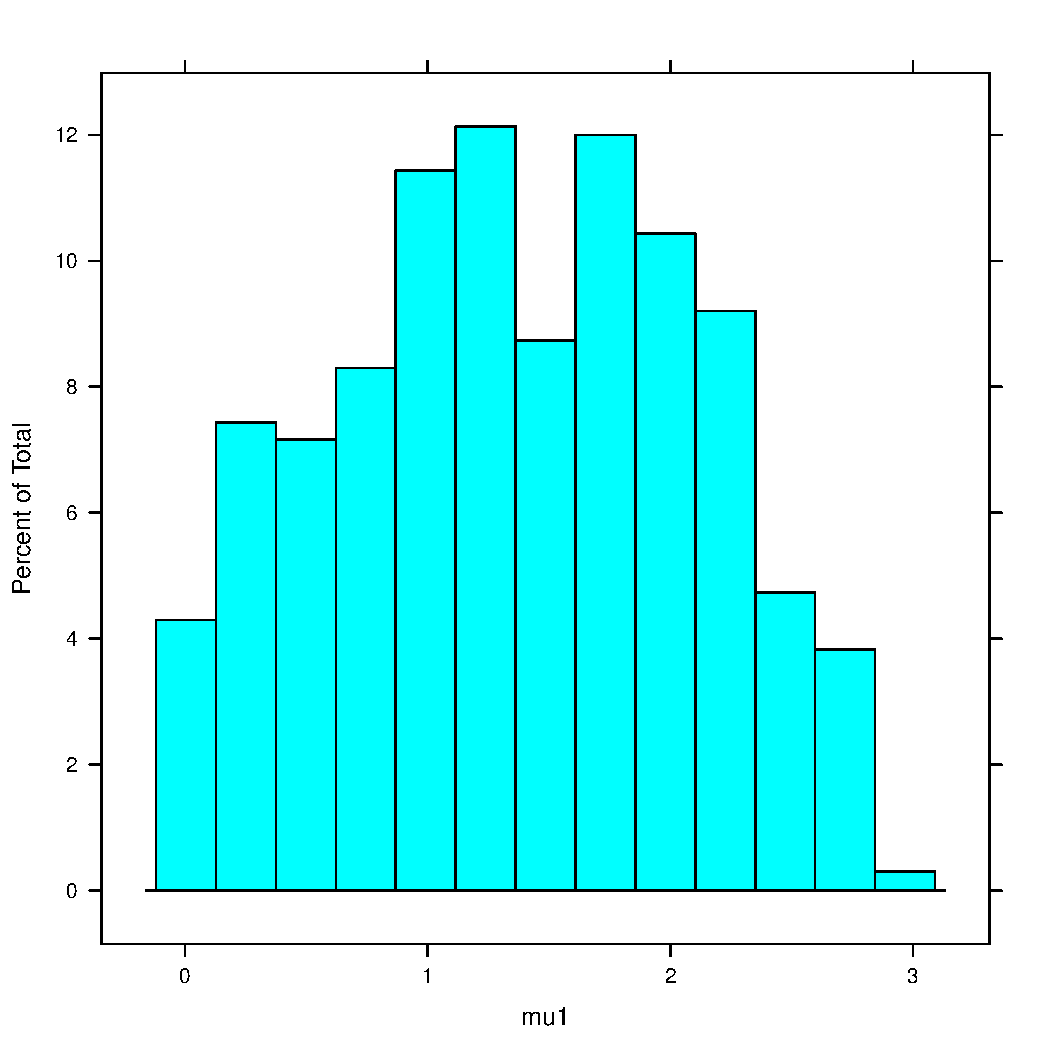
\includegraphics[scale=0.4]{mu1.pdf}
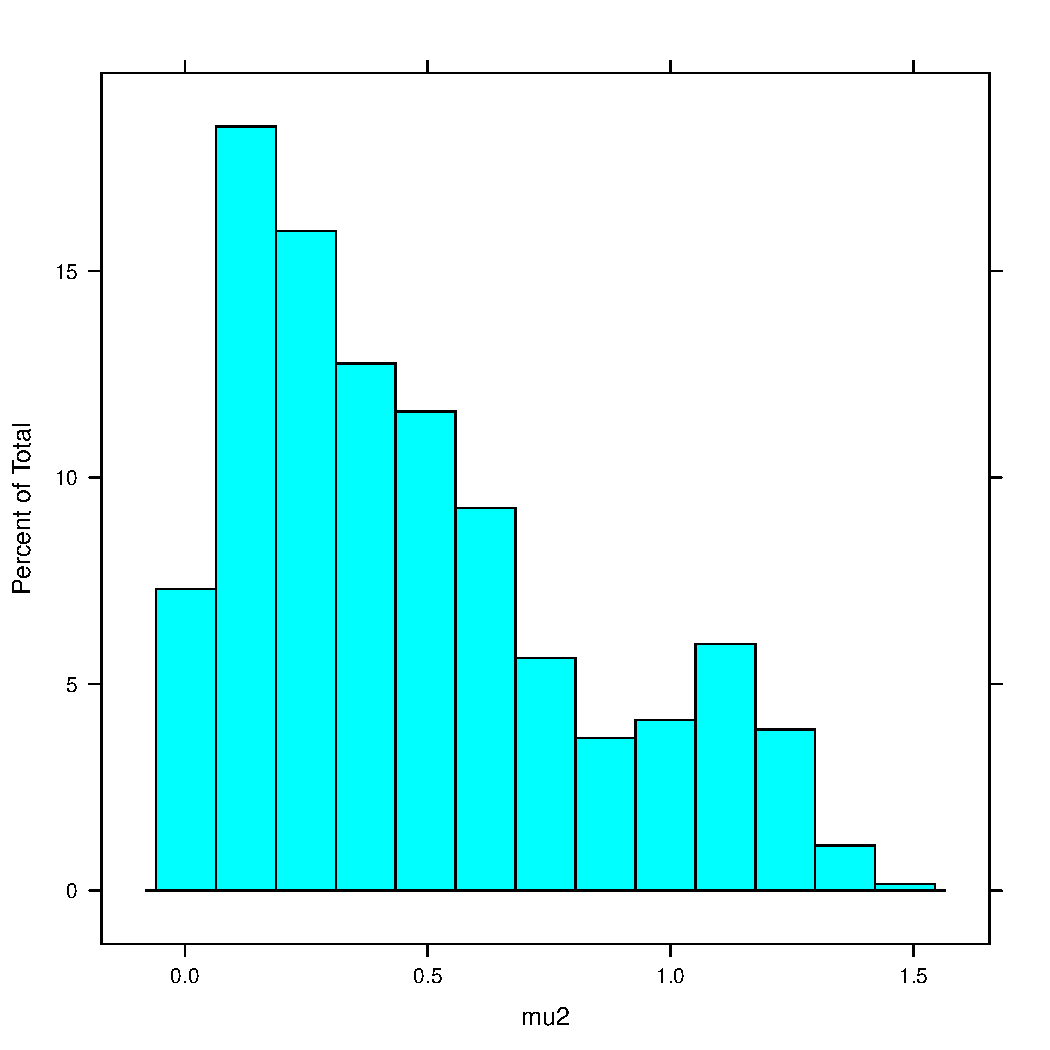
\includegraphics[scale=0.4]{mu2.pdf}
\caption{Histogram of Posterior Samples}
\label{post-samps}
\end{center}
\end{figure}

\paragraph{F}

I would use a composite from all three samples, weighted by the posterior probability of each. For the data given, my estimates of these values are $\mu_1=1.80$, $\mu_2=3.30$, $\sigma_1=0.770$, $\sigma_2=0.316$. 


\end{answer}



\end{document}